\section{Platine A als Single-Tone Sender}
Für den ersten Teil des Versuchs werden zwei identische Transceiver-Platinen verwendet, die bereits im Verlauf dieses Praktikums genauer betrachtet wurden.
Die beiden Platinen haben folgende Spezifikationen (\textcolor{red}{X} steht hierbei dafür, dass der Jumper entfernt ist, 
\textcolor{green}{\checkmark} dass der Jumper gesetzt ist):

\begin{table}[h!]
    \centering
    \begin{tabular}{|c|c|c|c|}
        \hline
         & J1 & J2 & Funktion \\
        \hline
        Platine A & \textcolor{red}{X} & \textcolor{green}{\checkmark} & Sender \\
        Platine B &\textcolor{red}{X} & \textcolor{red}{\textbf{X}} & Empfänger \\
        \hline
    \end{tabular}
    \caption{Spezifikationen der beiden Platinen}
    \end{table}
Die folgenden Abbildungen 4.1 und 4.2 zeigen auf der linken Seite die Platine B als Empfänger und auf der rechten Seite
die Platine A als Sender. Die beiden äußeren Lampen am USB-Port leuchten, sobald eine Versorgungsspannung
anliegt. Ist der Sender und Empfänger innerhalb der Funkreichweite, so leuchtet weder die Lampe TX (Transmitting) noch die Lampe RX am Sender und Empfänger.
Ist die Funkreichweite überschritten, so leuchtet die Lampe RX am Sender, die Lampe TX leuchtet nicht. Die Lampen
TX und RX am Empfänger sind unverändert.

\begin{figure}[H]
    \centering
    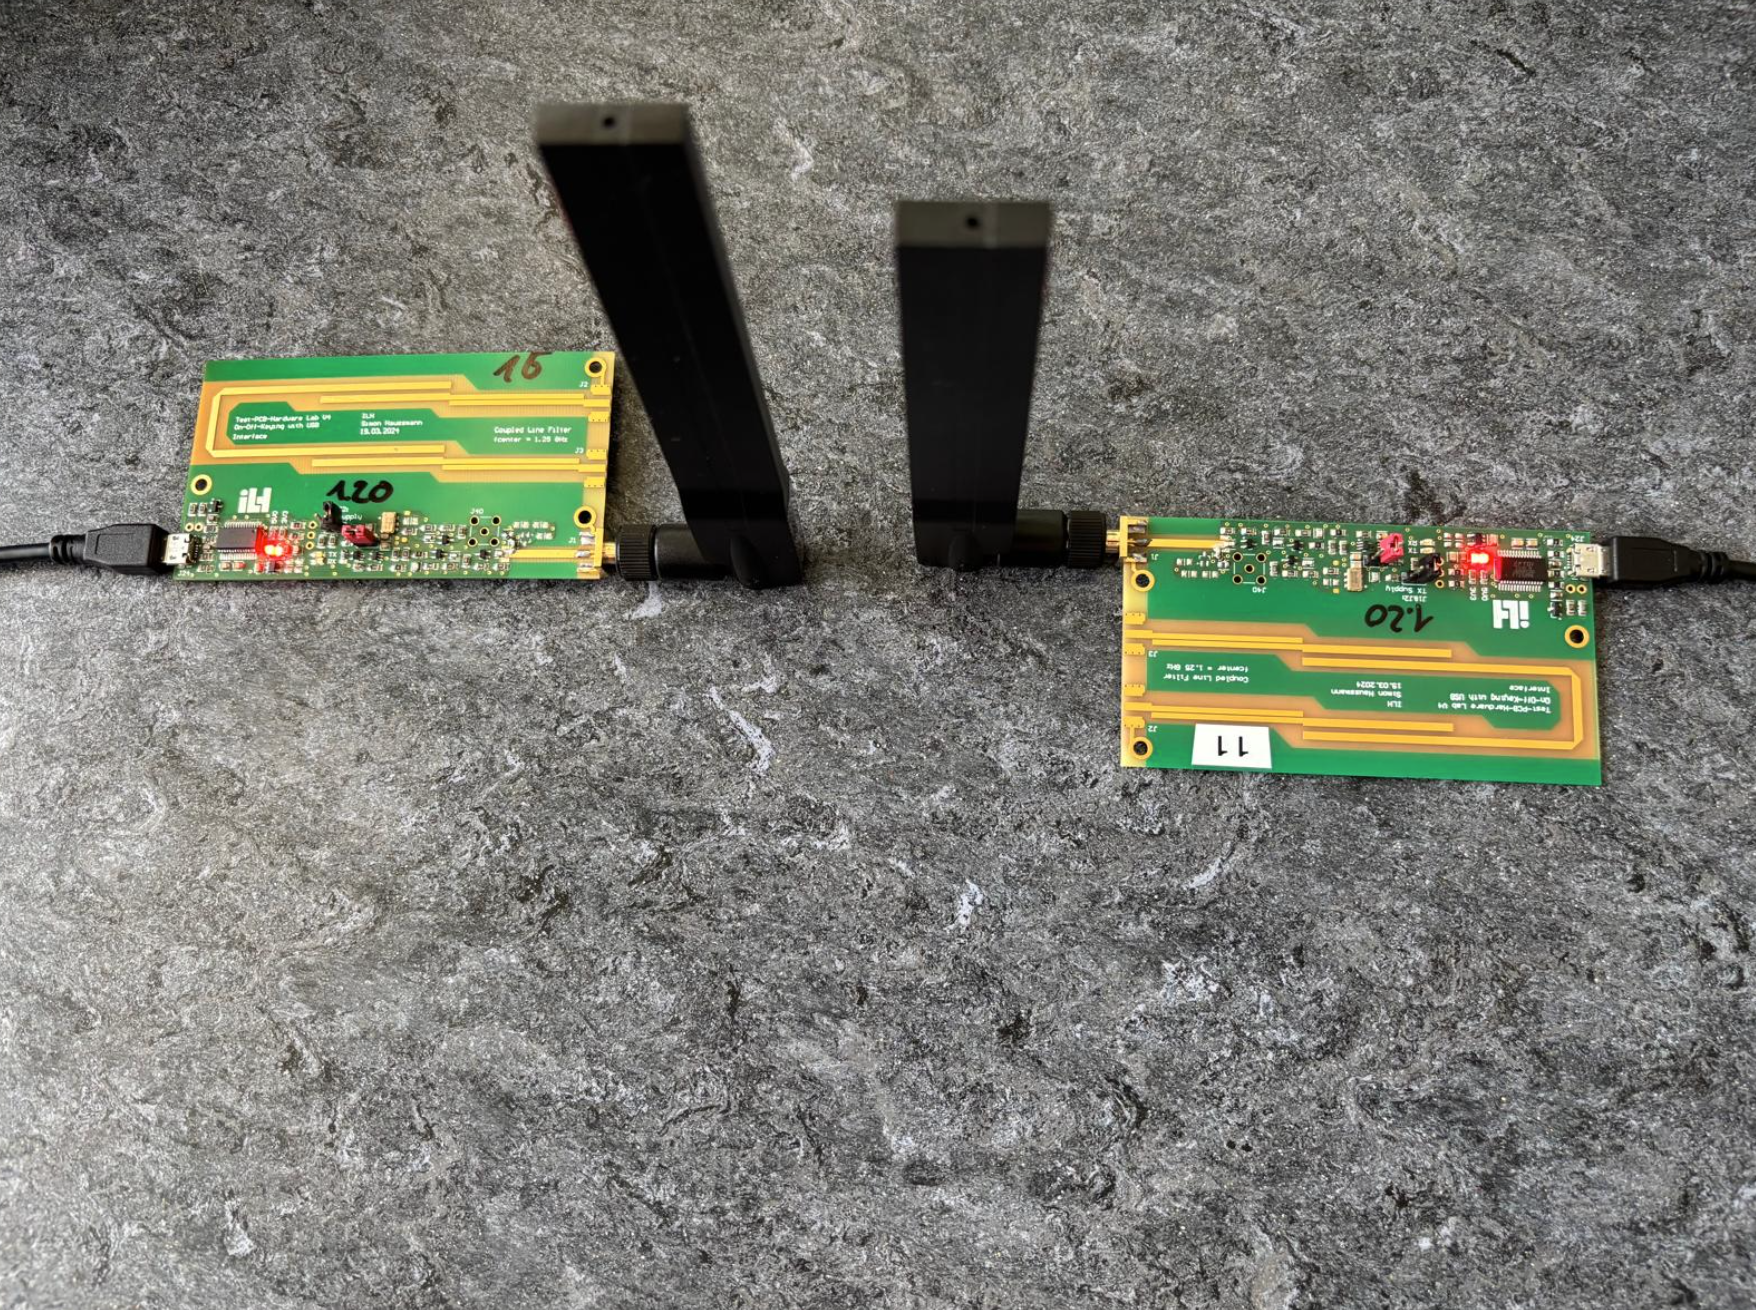
\includegraphics[width=0.6\textwidth]{Pictures/Task2a.png}
    \caption{Sender und Empfänger innerhalb der Funkreichweite}
    \label{fig:Task2a}
\end{figure}

\begin{figure}[H]
    \centering
    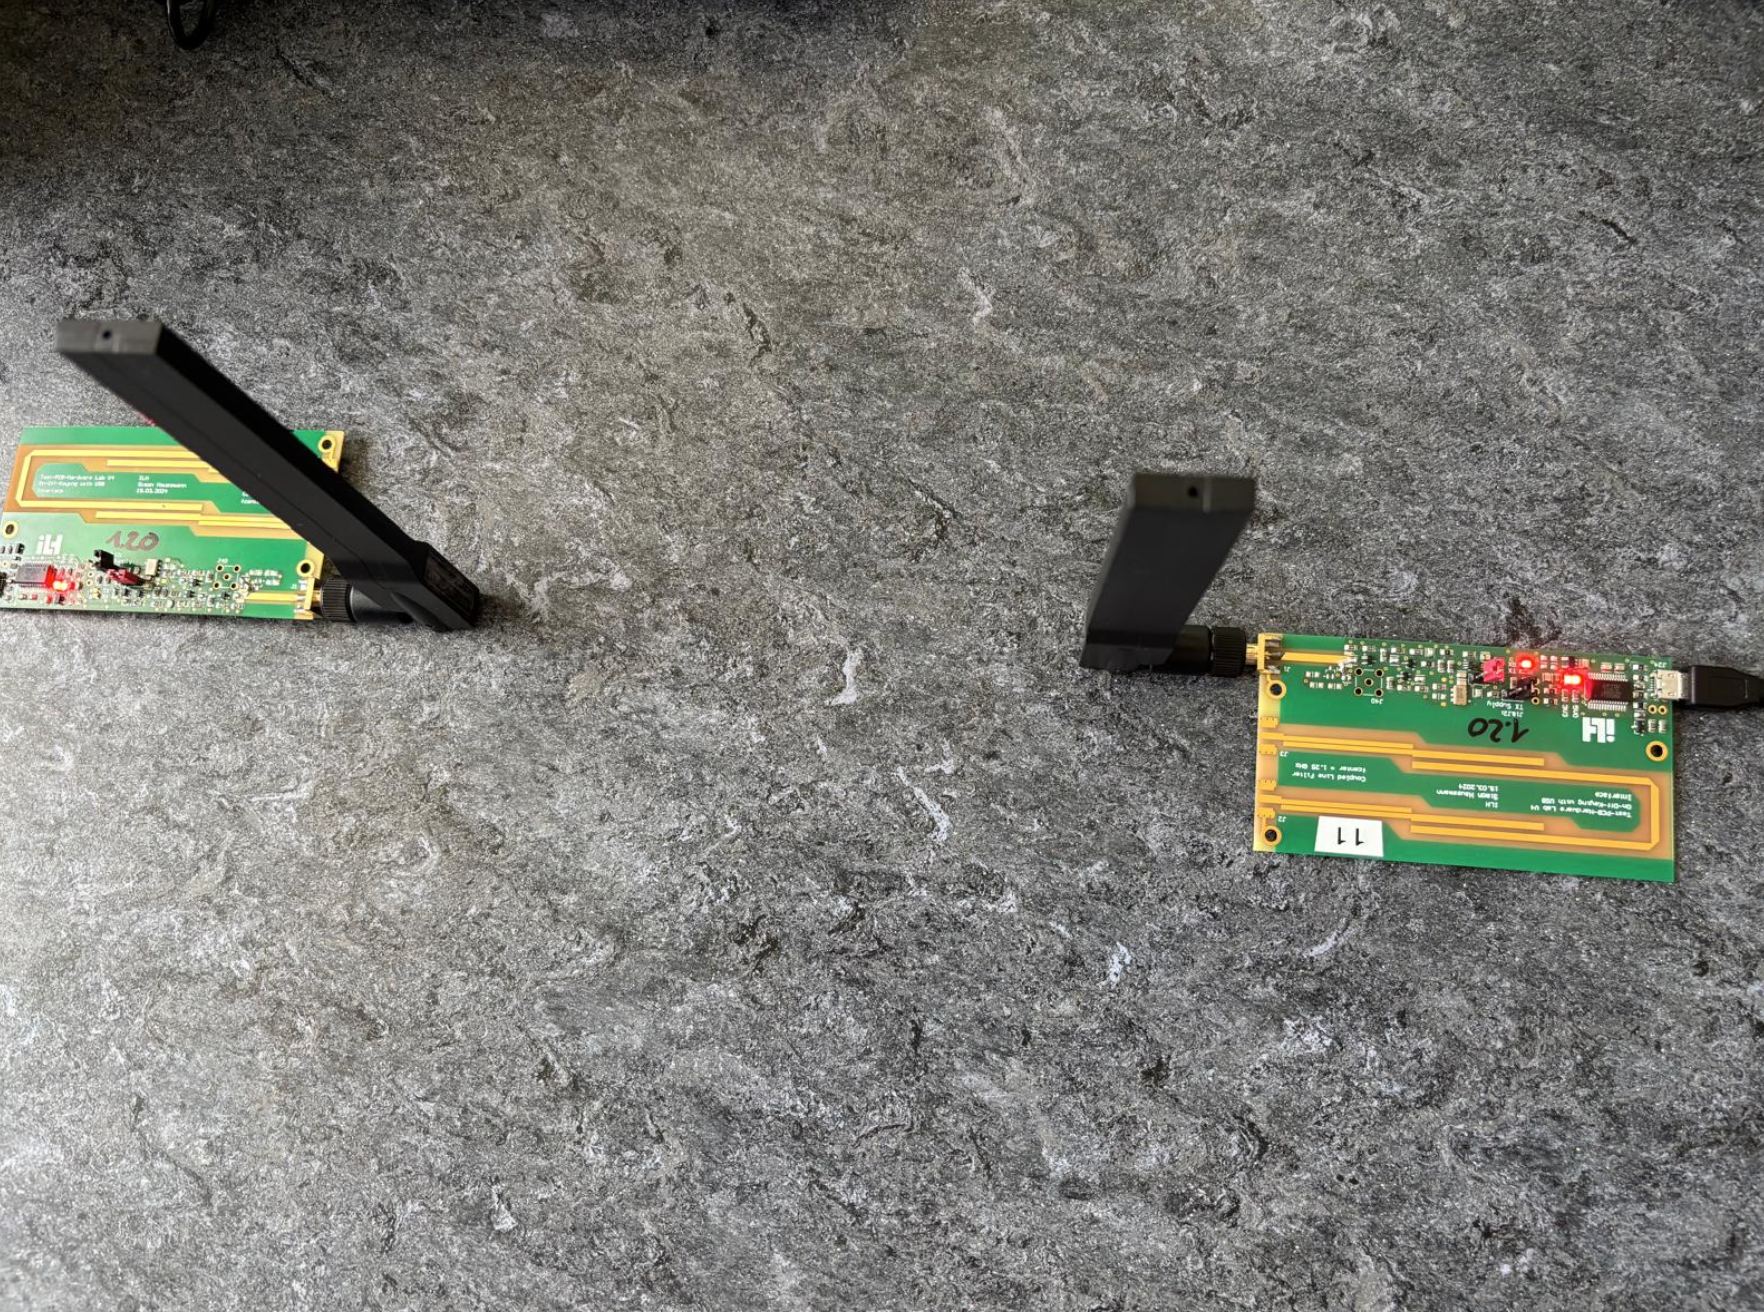
\includegraphics[width=0.6\textwidth]{Pictures/Task2aa.png}
    \caption{Sender und Empfänger außerhalb der Funkreichweite}
    \label{fig:Task2aa}
\end{figure}

\section{Platinen am Computer anschließen}
Nun wurde eine Platine an den Computer angeschlossen und die andere Platine an den Laptop.
Mithilfe von Hterm werden Daten in Form von ASCII-Zeichen von der einen Platine an die andere gesendet
und mit Hterm wieder ausgelesen.
Wichtig in dieser Prozedur war das Verbinden beider Jumper an der Sender-Platine und das Entfernen beider
Jumper an der Empfänger-Platine. 
Wären die Jumper bei der Empfänger-Platine verbunden gewesen, wäre das Problem gewesen, dass die Platine auch 
ein Signal gesendet hätte und dieses auch wieder empfangen hätte, was unerwünscht ist.
In der Praxis konnten wir mit diesem Setup eine nutzbare Reichweite von etwa 7,5 cm erreichen.

\section{Interessante/Witzige Beobachtung}
Als wir die Messung von Task4 durchgeführt haben und dann bei größeren Entfernungen kein Signal mehr erfasst hatten,
haben wir aus Spaß einen Samsung-Pen auf beide Antennen gelegt und aufeinmal konnten wir wieder Signale empfangen.
Ein möglicher Grund dafür könnte sein, dass der Samsung-Pen metallische Bestandteile enthält,
die die EM-Welle besser leiten als Luft.

\begin{figure}[H]
    \centering
    \includegraphics[width=0.4\textwidth]{Pictures/stift.png}
    \caption{Samsung Pen auf Antenne}
\end{figure}